\begin{figure}[!hp]
  \begin{center}
    \begin{tikzpicture}
      \begin{axis}[
          %colorbar,
          hide axis,
          scale only axis,
          height=0.41\rasterimagewidth,
          width=\rasterimagewidth,
          %colorbar horizontal,
          point meta min=2.55,
          point meta max=3.08,
          colorbar style={
            title=Concentration [\%w],
            width=7.4cm,
            height=0.3cm,
            xtick={2.5,2.55, 2.75, 3, 3.08, 3.5, 4, 4.5, 5, 5.5, 6},
            at={(0.5\rasterimagewidth,0.4cm)},
            anchor=north
          }
        ]
        \addplot [] coordinates {(0,0)};
        \node (myfirstpic) at (0,0) {\framebox{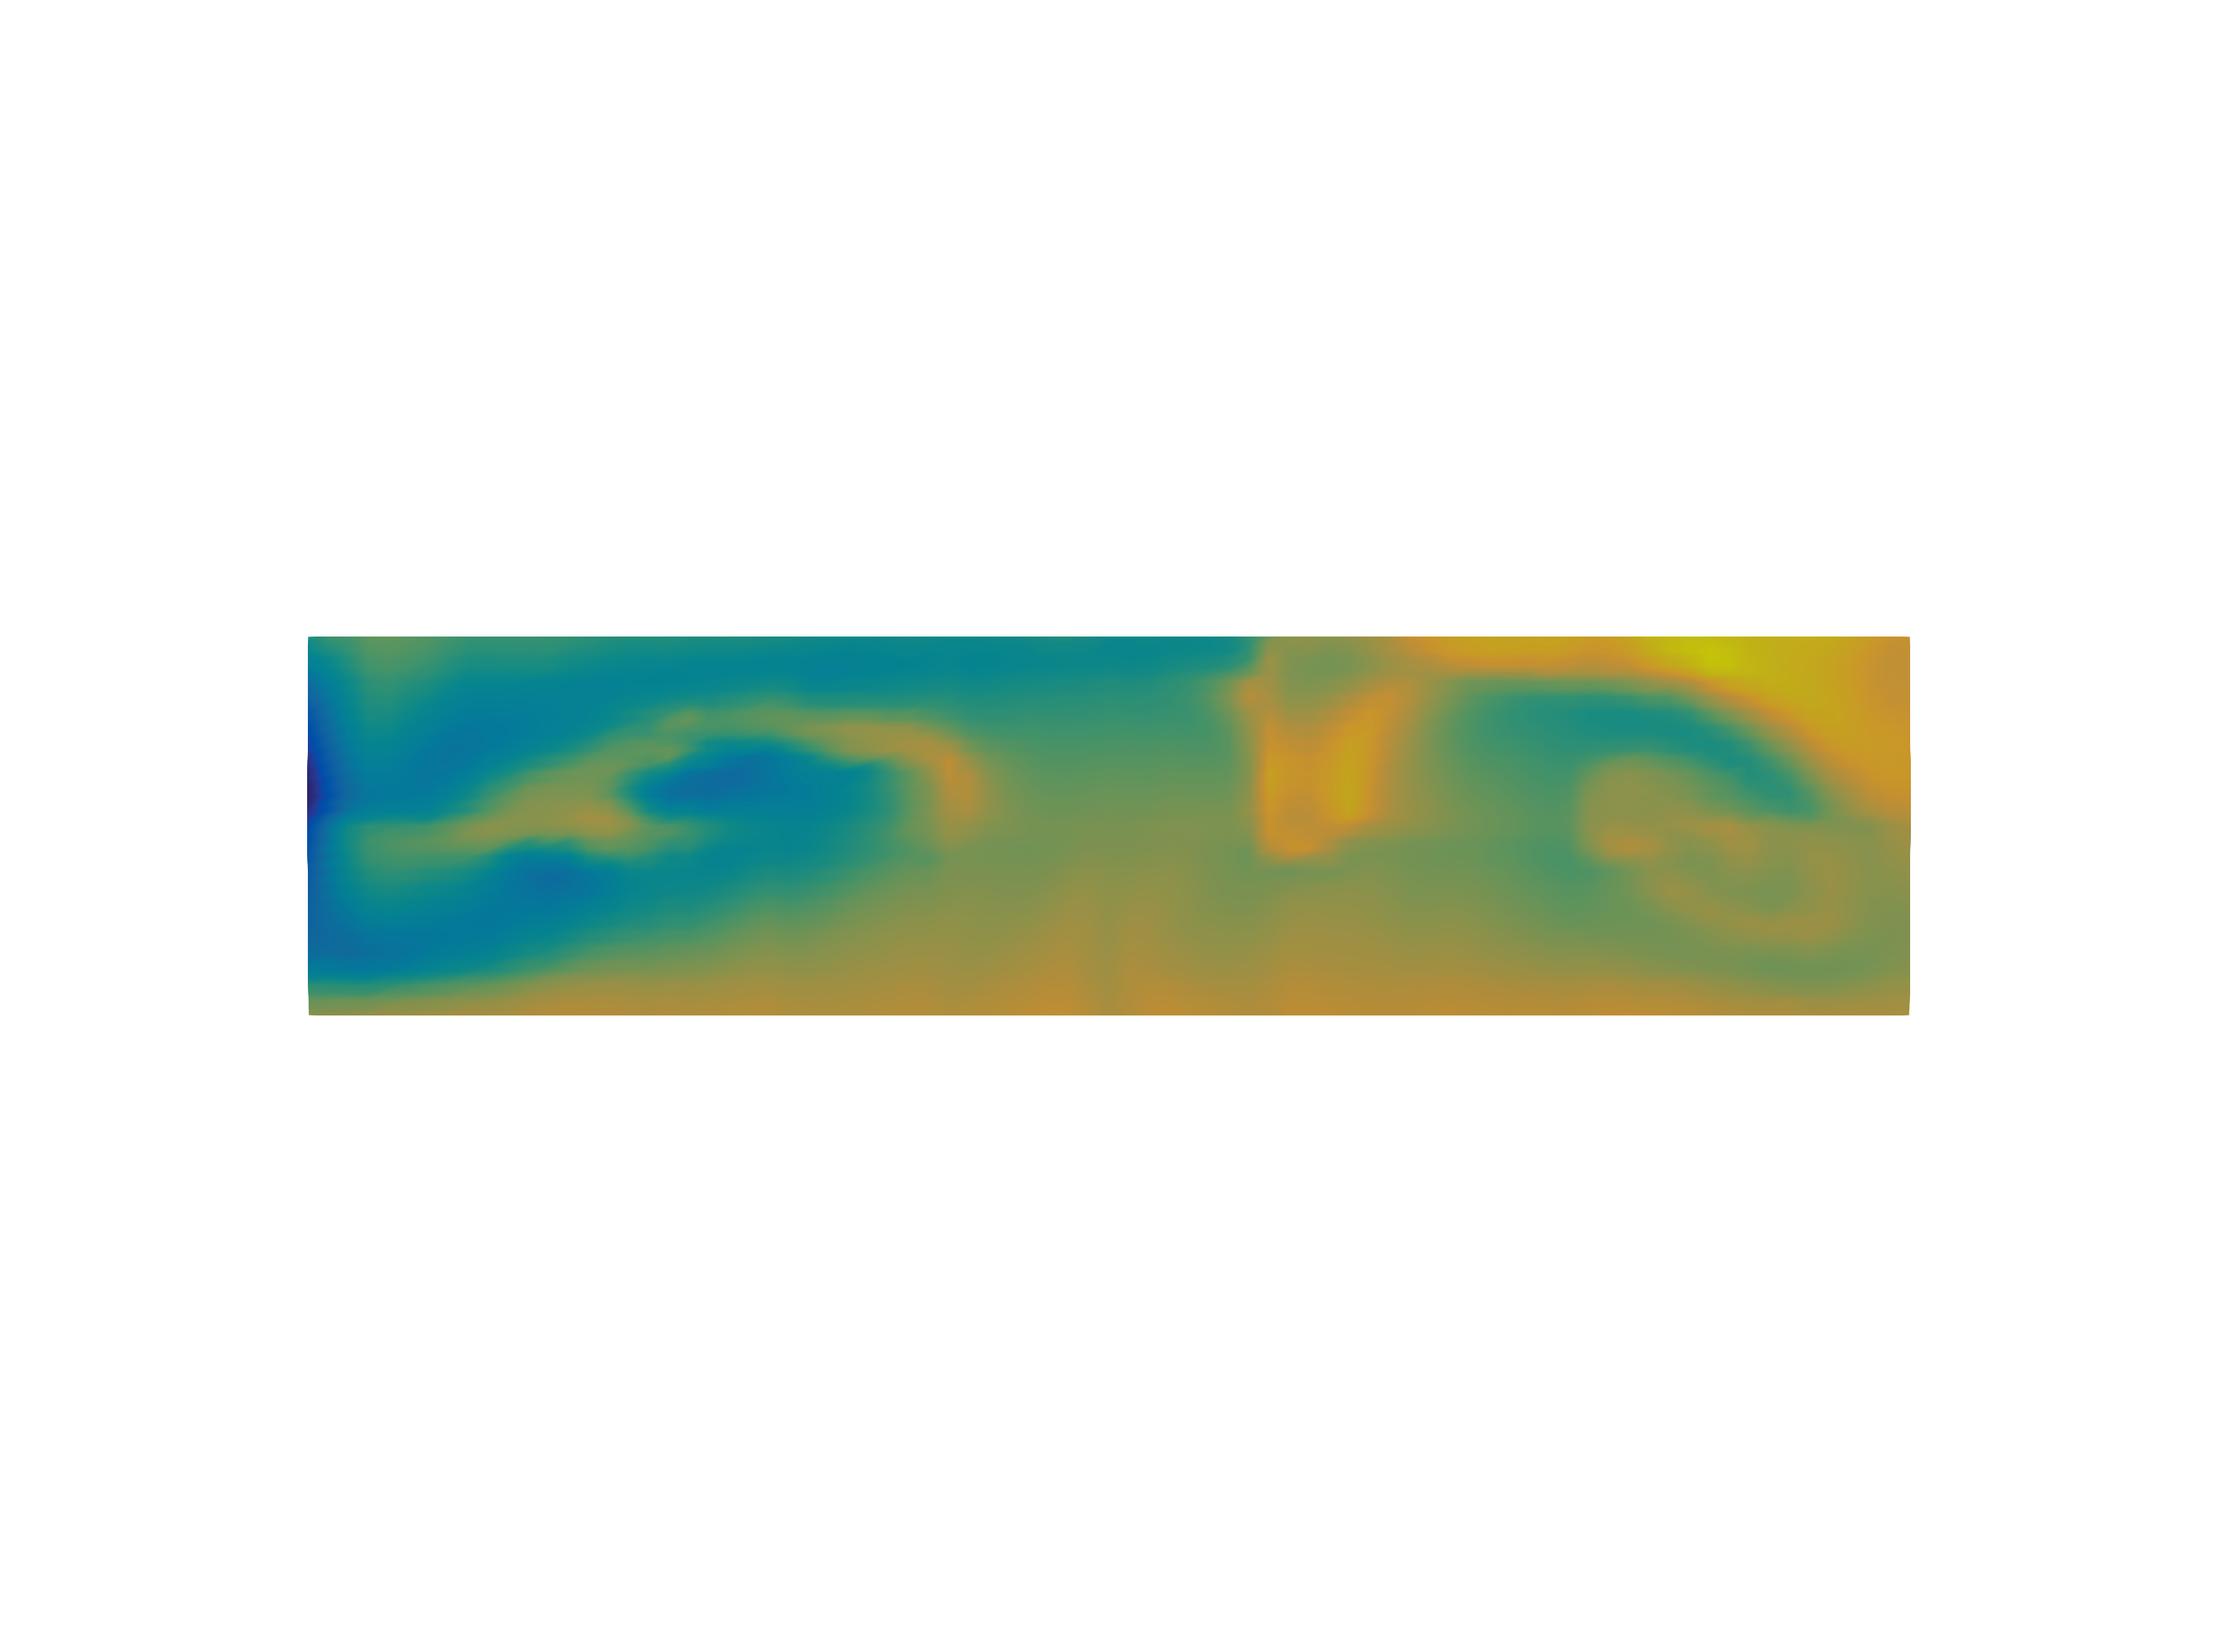
\includegraphics[width=\rasterimagewidth]{{../media/populations/application/print/alumina-influance-heaviside-2.55-3.08}.png}}};
      \end{axis}
    \end{tikzpicture}
    \begin{tikzpicture}
      \begin{axis}[
          colorbar,
          hide axis,
          scale only axis,
          height=0.41\rasterimagewidth,,
          width=\rasterimagewidth,
          colorbar horizontal,
          point meta min=2.55,
          point meta max=3.08,
          colorbar style={
            title=Concentration [\%w],
            width=7.4cm,
            height=0.3cm,
            xtick={2.5,2.55,2.75, 3,3.08, 3.5, 4, 4.5, 5, 5.5, 6},
            at={(0.5\rasterimagewidth,0.4cm)},
            anchor=north
          }
        ]
        \addplot [] coordinates {(0,0)};
        \node (myfirstpic) at (0,0) {\framebox{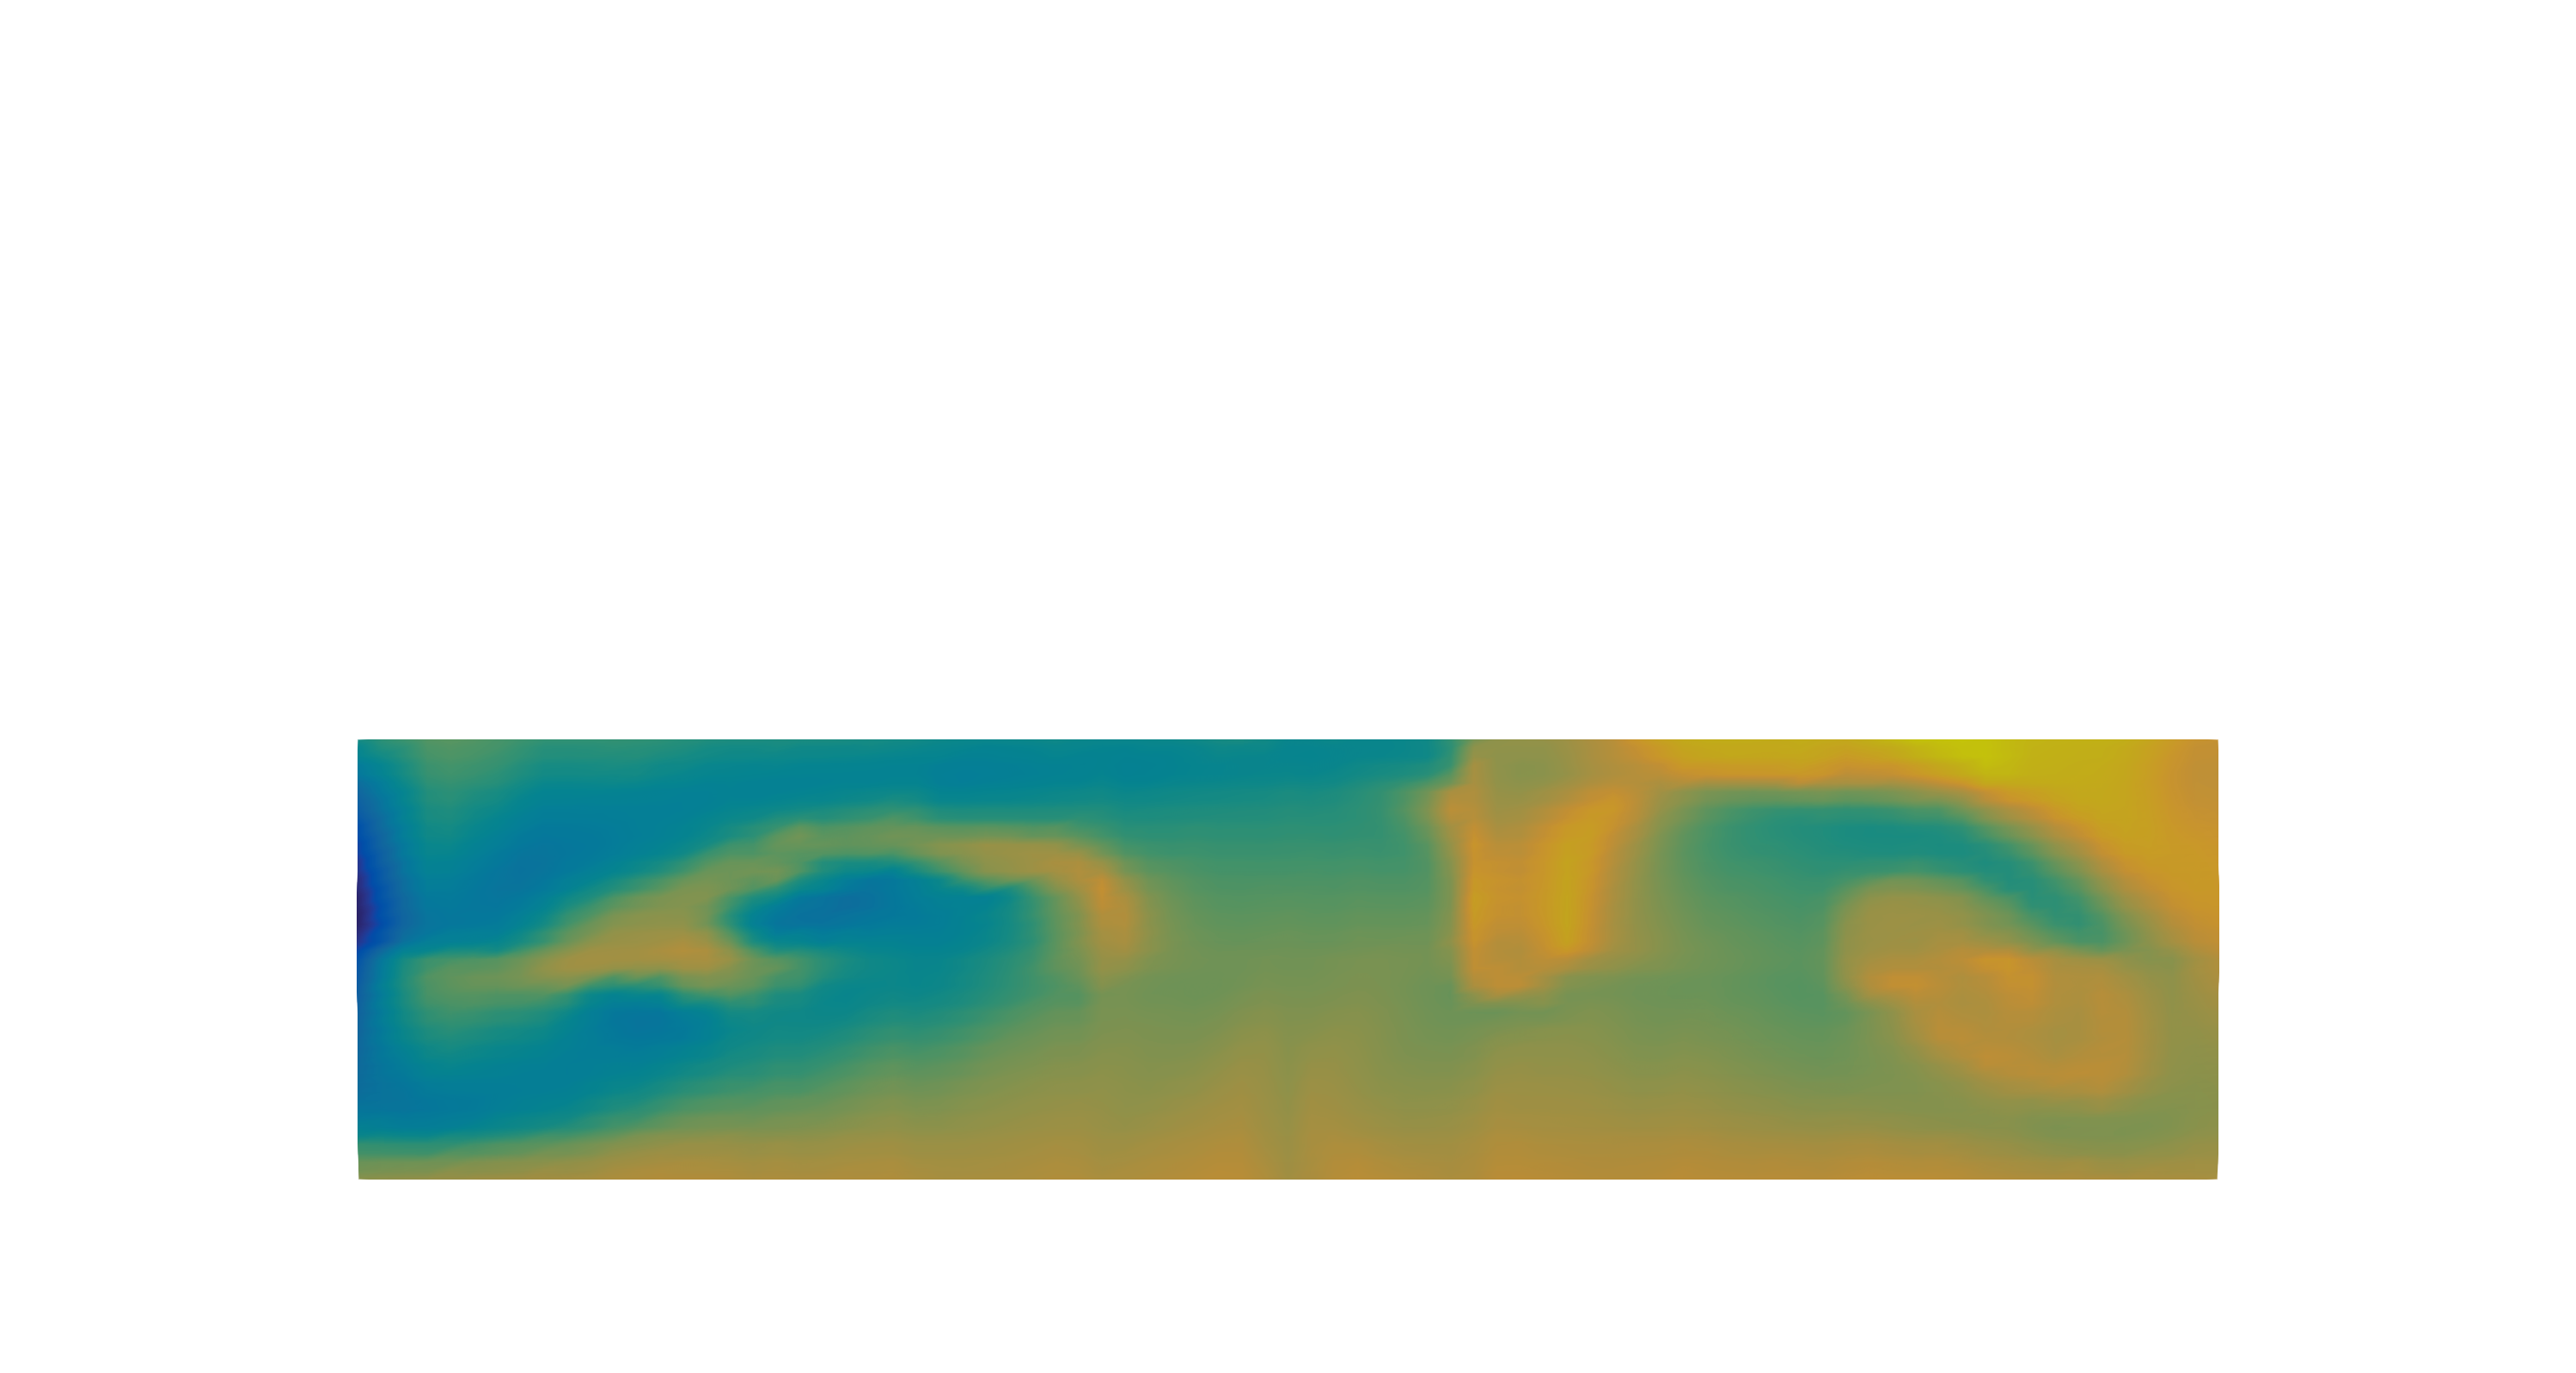
\includegraphics[width=\rasterimagewidth]{{../media/populations/application/print/alumina-influance-exp-2.55-3.08}.png}}};
      \end{axis}
    \end{tikzpicture}
    \caption{Champ de concentration $c$ dans l'ACD de la cuve AP32 à
      $t = $ \num{10000} \si{\second}. En haut, $T_\text{Crit} =
      T_\text{Liq}$. En bas, $T_\text{Crit} = T_\text{Liq} + 0.86$
      \si{\kelvin}.}
    \label{fig:dissolution-influence-exp-heaviside}
  \end{center}
\end{figure}
